% Contoh pembuatan persamaan
\begin{equation}
    \label{eq:hukumpertamanewton}
    \sum \mathbf{F} = 0\; \Leftrightarrow\; \frac{\mathrm{d} \mathbf{v} }{\mathrm{d}t} = 0.
\end{equation}


% Contoh input gambar
\begin{figure}[ht]
    \centering

    % Ubah dengan nama file gambar dan ukuran yang akan digunakan
    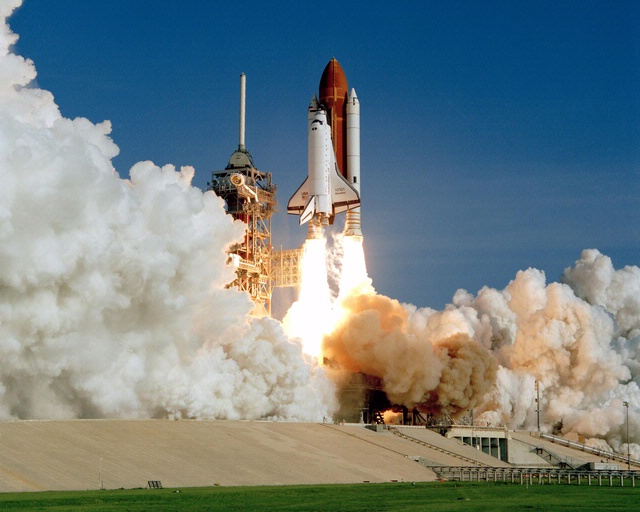
\includegraphics[scale=0.35]{gambar/roketluarangkasa.jpg}

    % Ubah dengan keterangan gambar yang diinginkan
    \caption{Peluncuran roket luar angkasa \emph{Discovery} \citep{roketluarangkasa}.}
    \label{fig:roketluarangkasa}
\end{figure}

% Reference Gambar
\emph{Discovery}, Gambar \ref{fig:roketluarangkasa}, merupakan


% Contoh pembuatan potongan kode
\begin{lstlisting}[
    language=C++,
    caption={Program halo dunia.},
    label={lst:halodunia}
  ]
  #include <iostream>
  
  int main() {
      std::cout << "Halo Dunia!";
      return 0;
  }
\end{lstlisting}


% Contoh input potongan kode dari file
\lstinputlisting[
  language=Python,
  caption={Program perhitungan bilangan prima.},
  label={lst:bilanganprima}
]{program/bilangan-prima.py}